\documentclass{article}
\usepackage[utf8]{inputenc}

\title{Synthesising emotion-driven images using image emotion classifiers}
\author{Konrad Cybulski}
\date{April 2019}

\usepackage{natbib}
\usepackage{graphicx}

\begin{document}
	
\maketitle


\section{Introduction}

For centuries artists have been extremely talented at creating pieces of artwork that convey a range of emotions to those who view them.
Extensive research has been conducted into how visual features affect humans emotionally and how these can be used to predict and detect the emotional content of images and text \citep{machajdik2010affective, zhao2014exploring}.
Due to the subjective and qualitative nature of human emotion, assigning a quantitative measure of emotion to an image is no easy task.
Furthermore the ability to computationally recognise the emotional content of an image has wide-ranging applications from classifying posts on social media, to the creation of images, text, and even physical spaces in an emotionally quantifiable way.

This research aims to explore the use of neural network image emotion classifiers in synthesising emotionally-driven images.
Primarily exploring the patterns and visual characteristics of such generative systems in their ability to create emotionally-targeted images.
In doing so, compare categorical (happy, sad, etc.) and continuous (valence-arousal-dominance) representations for emotion in the context of both image classification, and synthesis.
Through the generative process, gain a better understanding of visual patterns learnt by such a classifier by maximising classification confidence through the use of conditional generative adversarial networks \citep{gauthier2014conditional}, and evolutionary techniques explored by \citep{nguyen2015deep}.

Methods for quantifiably representing emotion have been explored thoroughly in the domain of psychology, with continuous multi-dimensional models being used in lieu of a single emotional label.
The circumplex model of emotion introduced a two-dimensional space characterised by valence, and arousal; respectively representing positivity or negativity, and the level of excitement associated with it \citep{russell1980circumplex}.
Such a continuous model is not without flaw, failing to accurately capture more complex emotional states, often those that represent concurrent conflicting sides of a given axis \citep{larsen1992promises}.
The complexity of such a continuous representation of emotion has been investigated in depth and extended in various ways such as by \citet{bradley1994measuring}, through the addition of a third dimension: dominance; which is particularly of interest within social dynamics.

The domain of emotion classification has had a particular focus on facial expressions and text \citep{cambria2016affective, warriner2013norms}.
Image emotion classifiers have been explored \citep{kim2018building, machajdik2010affective, chen2015learning, chen2014deepsentibank} yet their use has been limited.
While humans ability to recognise, label, and discuss the emotive content of an image is not lacking, the capability to computationally classify image emotion, and the underlying patterns learnt by such classifiers is.

As with the use of deep neural network image classifiers such as ResNet, AlexNet, and Inception, the shapes and patterns learnt by such deep learning systems are difficult to extract.
Recent work has looked at the use of quality-diverse generative algorithms with such deep classifiers \citep{nguyen2015deep, nguyen2015innovation}.
The underlying patterns learned by the classifier can be surfaced by synthesising images that maximise various desirable features.
This method allowed the exploration of images to which the classifier assigns a given label such as \textit{school bus} or \textit{lighthouse}, enabling a deeper understanding of the visual characteristics inherent to each class.

\section{Aims and motivation}
The aim of this research is develop an image emotion classifier in order to produce a generative system to synthesise emotionally-driven images to better understand the visual patterns associated with emotions conveyed in images as learnt by such a classifier.
This will primarily leverage image emotion recognition architectures explored by \citet{kim2018building}, in combination with the dataset produced by \citet{zhao2016predicting} containing over 1.4 million images with assigned valence, arousal, and dominance levels derived from their descriptions.
Producing and comparing architectures with which valence-arousal (VA) values, or emotion labels can be assigned to images forms the basis for this research.

This base architecture enables the exploration into how VA values are assigned to more complex, multi-faceted and multi-layered images, and methods for incorporating this classifier into an image synthesis system.
A generative process for synthesising emotionally-driven images will be explored that utilises the image emotion classifier produced.
This generative system, and the patterns learned by it, will be better explored by maximising given target features in a quality-diverse way \citep{nguyen2015innovation, nguyen2015deep}, and through a conditional generative adversarial approach \citep{tan2017artgan, gan2017stylenet}.
In the context of this research, such features include valence, arousal, dominance, happiness, sadness, etc.
This will allow a greater understanding of the visual patterns that such an architecture learns, and any psychological or artistic parallels that can be drawn.
The combination of such a generative system with a classifier of emotion can be further extended to domains such as generative art and text-to-image synthesis, with a focus on emotion-driven image generation.

\section{Research questions}

\paragraph{How can an image emotion classifier be used to synthesise emotion-driven images?}
\begin{itemize}
	\item How can the emotional content of images be represented?
	\item What methods can be used in combination with an image emotion classifier to synthesise images?
	\item How can patterns and visual characteristics learnt by an image emotion classifier be explored?
\end{itemize}


\section{Background}

\subsection{Image emotion recognition}

The area of image emotion and sentiment classification has been explored in a number of ways, primarily through image feature analysis derived from art and psychological factors \citep{machajdik2010affective}; and more recently using techniques such as deep neural networks \citep{chen2015learning, kim2018building}.
Feature extraction and analysis has been used for various applications such as measuring aesthetic appeal \citep{den2010using,den2010comparing,den2011evolving} and as an emotional feature vector for sentiment classification \citep{machajdik2010affective}.
Due to the artistic and psychological underpinnings used by \citet{machajdik2010affective}, the low-level features extracted from images can be understood at a high level.
The relationship between an image's emotion and its core artistic components such as balance, harmony, and variety was further explored by \citet{zhao2014exploring}, which uses a comparably small feature vector to \citet{machajdik2010affective}, resulting however in a 5\% classification increase to state-of-the-art approaches at the time.

Deep neural networks in this domain provide less transparency to the process with which emotions and sentiment are classified compared to feature analysis.
The emotional content of an image can be decomposed in various ways.
Image databases with singular emotion labels, and adjective-noun pairs (ANP) have been used for the training of deep neural network classifiers \citep{chen2014deepsentibank, yang2018visual} with up to 200\% performance gains over support vector machine classifiers.

Given the large amount of work conducted into image object classification, producing neural networks such as AlexNet, ResNet, and Inception, transfer learning has been heavily relied upon in various domains of classification and synthesis from images.
Techniques used by image emotion recognition have been used extensively in domains such as image sentiment analysis \citep{you2015robust}, and image-to-text synthesis \citep{vinyals2015show}.
The subjectivity and human-dependent nature of emotion has naturally resulted in only small datasets of emotion-labelled images.
Through transfer learning, pre-trained image object classifiers can and have been used in the domain of image emotion \citep{kim2018building, wangarttalk}.

Sentiment is typically represented as a binary classification of either positive or negative \citep{yang2018visual, chen2014deepsentibank}.
Facial and image emotion classification however face a higher complexity problem, where research has typically focused on a subset of potential emotions ranging in size from 7 \citep{ali2017emotional}, 8 \citep{machajdik2010affective}, 11 \citep{wangarttalk}, and even 19 \citep{mohammad2018wikiart}.
Other methods for representing emotion include use of the circumplex model of affective emotion \citep{russell1980circumplex, bradley1994measuring}.
This model represents emotion as a continuous multi-dimensional space.
The original definition by \citet{russell1980circumplex} introduces a two-dimensional space defined by valence, and arousal.
Valence represents the positive and negative aspect of an emotion; arousal, the excitatory component.
In such a model, each emotion label used in common categorical classification resides within the space as seen in \ref{fig:valence-arousal}.
The circumplex model has been applied and extended in various ways.
The addition of a third dimension, dominance, introduced by \citet{bradley1994measuring} allowed the representation of emotion relating to feelings of situational control.
Despite the increased freedom of representation in a continuous space, problems exist with the circumplex model \citep{larsen1992promises}.
Some of the key issues with such a model is its dichotomous nature, resulting in a comparative failure to capture more complex emotions, particularly emotional states representing conflicting sides of a dimension.

\begin{figure}[h!]
	\centering
	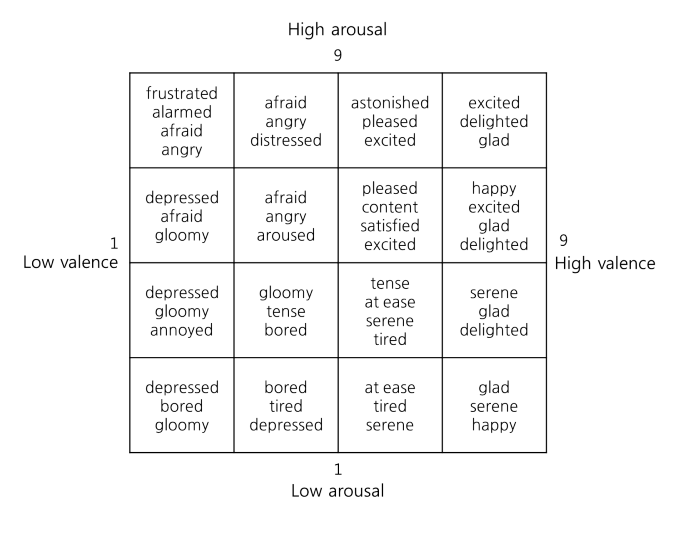
\includegraphics[width=0.75\textwidth]{images/valence-arousal-grid.png}
	\caption{Distribution of emotions associated with levels of valence and arousal determined by the DNN classifier produced by \citet{kim2018building}}
	\label{fig:valence-arousal}
\end{figure}

The use of continuous emotion representations, particularly relating to the circumplex model have been explored in image emotion recognition tasks \citep{kim2018building, zhao2016predicting, zhao2017continuous}.
Regression models produced to predict the valence-arousal (VA) values of given images have shown high accuracy on various datasets.
In leveraging pre-trained image classification networks through transfer learning, even smaller datasets (10,000 images) can have high accuracy classification results \citep{kim2018building}.
Recent datasets produced for image emotion recognition have used the valence-arousal-dominance model due to its continuity \citep{zhao2016predicting}.
While categorical classification is more easily verified by humans, training predictive models with data that has an element of noise and uncertainty benefits from both continuity and volume.
This is a key advantage of the circumplex model as applied by \citet{kim2018building} and \citet{zhao2016predicting} in image emotion recognition over categorical classification.


\subsection{Computational image synthesis}

\begin{figure}[h!]
	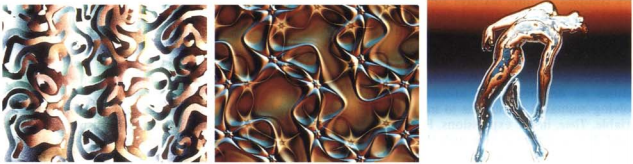
\includegraphics[width=\textwidth]{images/sims-interactive-image-generation.png}
	\caption{Images generated through the process of interactive evolution introduced by \citet{sims}}
	\label{fig:sims}
\end{figure}

Generative systems have been explored in various domains with numerous techniques.
Examples range from the generation of images and art using evolutionary methods \citep{sims, nevar}, to the synthesis of text to describe a given image through the use of deep neural networks \citep{mathews2016senticap}.
Some of the first \textit{human-in-the-loop} image synthesis systems such as \textit{NEvAr} \citep{nevar} produced greatly impressive images through evolutionary techniques.
Evolutionary art leveraged methods introduced and exemplified by \citet{sims} such as those shown in Figure \ref{fig:sims}.
\citet{sims} proposed using \textit{Lisp} expressions for genotype definitions, which accepted a coordinate (x, y) which could be evaluated into a grayscale or RGB value producing images.
This genotype expression has been used in numerous further research into the process of both supervised and unsupervised image synthesis through evolutionary techniques \citep{nevar, sims, den2011evolving, distributed-evolutionary-art, aesthetic-measures}.

Despite the slow nature of the interactive process, \citet{sims} and \citet{nevar} were able to produce images with visually striking characteristics.
\citet{aesthetic-measures} investigated measures of aesthetics for fitness evaluation in artificially evolving images.
This research primarily used observations by \citet{ralph-bell-curve}, that the distribution of colour gradients in fine art tend towards normal.
While the images produced through this method did not meet the level of intricacy and detail as the results of \citet{sims} or \citet{nevar}, it represented a self-contained system able to generate appealing imagery without human interaction.

Introduction of the generative adversarial network architecture (GAN) by \citet{GAN} allowed the process of image generation to depend only on collecting a sufficiently large dataset.
Common GAN application has involved the generation of realistic images, such as has been done by \citet{bao2017cvae}, where images have been synthesised to fine-detailed target labels such as bird species' and actors.
\citet{zhang2017stackgan} and \citet{reed2016generative} have recently explored text to image synthesis, in which detailed descriptions of birds and flowers have been converted into photo-realistic images using the GAN model.
Such an architecture has been applied to the area of art synthesis by \citet{tan2017artgan} in which images were generated according to a target genre and artist.
Learning from a dataset of countless artworks under various categories, styles, and artists, it was hugely successful in generating images that were stylistically similar to existing art of the target artist/genre.
Due to the competitive relationship of the generator and discriminator networks, the patterns learned by the discriminator propagate through the generator network.
The discriminator network of the GAN architecture aims to learn patterns and styles from the dataset on which it is trained in order to discriminate between the generated and existing images.
As a result, the images generated tend to resemble closely those in the training dataset, which represents a benefit in successfully producing images closely matching the target domain, and a detriment with regard to the networks potential creativity.

Recent work by \citet{nguyen2015innovation} and \citet{nguyen2015deep} investigated the use of quality-diverse algorithms for image generation particularly to better understand the patterns learned by deep neural network image classifiers.
Quality-diverse (QD) evolutionary algorithms such as Multi-dimensional Archive of Phenotypic Elites (MAP-Elites) \citep{mouret2015illuminating} and Novelty Search \citep{lehman2008exploiting, lehman2011abandoning} have been developed to address the need for a high quality, yet diverse solution space in related optimisation domains.
The use of such QD algorithms has shown great promise in its efficiency and accuracy on a number of hard optimisation problems \citep{pugh2016quality} such as maze navigation \citep{lehman2011abandoning}.
\citet{nguyen2015deep} and \citet{nguyen2015innovation} use MAP-Elites in conjunction with a pre-trained deep neural network (DNN) image classifier; assigning individual image fitness according to the accuracy with which it is classified.
Using the MAP-Elites framework in this context, each dimension of the feature-space represents a classification label, and as such the generated images allow the exploration of label representative patterns and shapes learnt by the classifier.
\citet{nguyen2015deep} leverages such an architecture to show the shallowness with which an image classifier recognises images.
Assigning the label of \textit{school bus} to alternating yellow and black lines is a prime example of the way such a network has learnt to differentiate one class from the others.
Thus enabling exploration into the inner workings of the DNN classifier by uncovering features that maximise the separation of one label to another.
In contrast, \citet{nguyen2015innovation} uses the same architecture to explore the novelty-driven evolutionary path taken by generated images and the potential for such a system in the field of content synthesis.
While the conclusions derived from \citet{nguyen2015innovation} and \citet{nguyen2015deep} contrast greatly, the quality-diverse generative method used to understand the visual components learnt by the classifier show such an architecture's exploratory abilities.
This technique for understanding the patterns learnt by such a classifier has not been explored in the context of regression.

The application of generative systems in the domain of affective computing, particularly with regard to emotion and content synthesis, is limited.
Sentiment-driven examples of generative systems include image captioning according to target sentiment \citep{mathews2016senticap}.
The task of describing an image was extended from a traditional GAN approach through the addition of an sentiment target input.
The method used to train such a generative system involved the conditional GAN architecture as described by \citet{gauthier2014conditional}.
A similar technique was used in style-driven image captioning (factual, romantic, humorous) in combination with a long short-term memory (LSTM) neural network model \citet{gan2017stylenet}.
In the context of image-to-image synthesis, \textit{emotion transfer} was explored by \citet{ali2017emotional} which involved the transformation of an image's colour and style with the aim of altering its conveyed emotion.

\section{Methodology}

\subsection{Emotion representation and prediction}
Method for representing emotion in this research have been limited to three options based on the dataset: a single categorical label (happy, sad, etc.); a two-dimensional circumplex model (valence-arousal); and a three-dimensional circumplex model (valence-arousal-dominance).
A model commonly used for representing emotion in classification tasks is that of a single categorical label, due its simplicity.
While this model represents a reductionist view of emotion, omitting a great deal of complexity, it will be the emotional representation used in this investigation.
Investigating the applicability of this simplistic model enables comparison between categorical and continuous representations of emotion explored in this work.
The more complex models investigated in this research include both the two and three dimensional circumplex models: valence-arousal, and valence-arousal-dominance respectively.
Each of these three models will be used as the classification/regression target of a deep neural network (DNN) model.

The DNN model architectures tested will be based on commonly used techniques such as those explored by \citet{kim2018building, chen2015learning}.
This technique, known as transfer learning, involves the repurposing of pre-trained DNN image classifiers by replacing or feeding through the final layers to another network.
The altered topology has the desired output shape and is able to proceed with further training in the given problem domain.
Initial investigation into the classification of image emotion will involve the use of such pre-trained DNN classifiers as ResNet, AlexNet, Inception, and VGGNet.
Further feature extraction and ensemble methods may be explored, particularly those investigated by \citet{kim2018building}, \citet{chen2015learning}, and \citet{chen2015learning}.
The accuracy of architectures will be compared within the context of each emotional representation, and between them.

\subsection{Image synthesis}
Having produced an image emotion classifier, this research will then focus itself on developing an emotion-driven image generation system to both generate images, and explore the underlying patterns and shapes learnt by the predictor network.
Following from work by \citet{nguyen2015innovation} and \citet{tan2017artgan}, this research will explore both the evolutionary quality-diverse algorithm MAP-Elites, in addition to neural networks for image synthesis.

In exploring the use of MAP-Elites for image generation, the system architecture used bases itself heavily on that introduced in \citet{nguyen2015innovation}.
The feature-space is explored through the evolution of direct image representations, allowing crossover and mutation of individual and collections of pixel values, evaluating fitness according to the accuracy with which the image is classified.
Given the quality-diverse focus of the MAP-Elites algorithm, the output will be a multi-dimensional space containing generated images distributed according to their label and classification accuracy.
The multi-dimensional regression model spanning the valence-arousal-dominance (VAD) coordinate space however cannot be explored in the same way since there is no classification accuracy with which to assign fitness.
The MAP-Elites algorithm will be applied in a similar way to investigate the use of such an evolutionary image synthesis method for later comparison.
In this context, fitness evaluation will be computed using the error between target VAD values and those determined by the classifier.

The other method explored for image synthesis involves training a conditional generator neural network following from work by \citet{tan2017artgan} and \citet{gauthier2014conditional}.
This process involves the training of a network that accepts as input: noise, and a condition.
The condition with which this network is trained represents the target emotion of the generated image.
This proposed architecture is trained to minimise error between the target emotion and that predicted by the classifier.
There exists the option to use networks pre-trained on other datasets for the generator network, as is explored by \citet{nguyen2016synthesizing}.
In doing so, enabling the generation of emotionally-driven images specific to a given domain.

In order to verify the system for emotion-driven image synthesis, the images generated by it will be involved in a human-validation process.
This will involve a sample of generated images having VAD values assigned to them using the self-assessment manikin \citep{bradley1994measuring} and the analysis of how human-attributed values compare to those intended by the system.

\subsection{Exploring emotion-specific patterns learnt by the image classifier}

A process for image synthesis conditioned on a target emotion enables the exploration of generated images with regard to their emotion-differentiating patterns and visual characteristics.
Techniques used by \citet{nguyen2015deep} and \citet{nguyen2015innovation} to explore DNN image classifiers involved the MAP-Elites algorithm; generating images that maximise classification accuracy as discussed in \textit{Background}.
While these techniques used the MAP-Elites algorithm, the process of exploring the feature-space through image synthesis can also be completed by the neural network approach mentioned.
The generative system produced as part of this research aims to generate images within a feature-space, that minimise the classification/regression error in order to better understand some key visual patterns and characteristics learned by the predictive network.
Since generative systems trained on given sets of data tend toward generating images similar to its training data, this generative exploration aims to incorporate as little prior learning into the process.

\section{Timeline}

\begin{table}[h!]
	\newcommand\tl[2]{
		\parbox[b]{8em}{\hfill{\bfseries #1}~$\cdots$~}\makebox[0pt][c]{$\bullet$}\vrule\quad \parbox[c]{6.5cm}{\vspace{7pt}\raggedright #2.\\[7pt]}\\[-3pt]
	}
	\centering
	\begin{minipage}[t]{.9\linewidth}
		\rule{\linewidth}{1pt}
		
		\centering \textbf{Semester One} \par
		
		\rule{\linewidth}{.7pt}%
		\tl{Week 6}{Research proposal}
		\tl{Week 9}{Literature review draft}
		\tl{Week 12}{Literature review}
		\tl{Week 13}{Compilation of data, ready for experimentation}
		\tl{Week 14}{Interim presentation}
		\rule{\linewidth}{.7pt}
		
		\centering \textbf{Semester Two} \par
		
		\rule{\linewidth}{.7pt}%
		\tl{Week 3}{Emotion representation predictive models trained}
		\tl{Week 4}{Comparison of image emotion predictive models completed}
		\tl{Week 6}{Image synthesis systems created and content produced for human-validation}
		\tl{Week 8}{Human validation of synthesised images complete}
		\tl{Week 10}{Further exploration of patterns learnt by classifier through generative exploration}
		\tl{Week 12}{Thesis completion}
		\tl{Week 14}{Final presentation}
		\bigskip
		\rule{\linewidth}{1pt}%
	\end{minipage}%
\end{table}



\section{Expected Outcomes and Contributions}

The initial outcome of this project is an image emotion classification system.
Multiple types of emotional representation are explored with reference to the classifier, both categorical emotion labels, and continuous multi-dimensional representations of valence, arousal, and dominance.
Comparisons between the accuracy of representations with respect to the classification domain will be explored, as will the comparative performance of various network architectures used in the transfer learning approach.
This section of the research will produce a usable, generalised, and extensible image emotion classifier.

The primary outcome of this research is the creation of an emotion-driven image synthesis system.
It will have been developed exploring various generative methods as discussed in \textit{Methodology}, and comparisons between them will be produced.
The generative process will be computationally validated in its ability to generate images according to a target emotion, in addition to being validated by humans using methods for measuring affective emotion.
The extensibility of techniques used for developing the image generator, particularly related to transfer learning from pre-trained image generators, will also be explored.
The content produced by the generative system in order to explore and better understand the visual components learnt by the classifier will be qualitatively analysed with respect to technical, artistic and psychological image features as introduced by \citet{machajdik2010affective}.
The synthesised images from the system developed will be exhibited to validate the efficacy with which it is able to produce targeted affective images.

\bibliographystyle{apalike}
\bibliography{references}

\end{document}
